\documentclass{article}

\PassOptionsToPackage{numbers,compress}{natbib}

% NeurIPS 2025 style, preprint mode for arXiv.
\usepackage[preprint]{neurips_2025}

\usepackage[utf8]{inputenc}
\usepackage[T1]{fontenc}
\usepackage{hyperref}
\usepackage{url}
\usepackage{booktabs}
\usepackage{amsfonts}
\usepackage{amsmath,amssymb}
\usepackage{nicefrac}
\usepackage{microtype}
\usepackage{xcolor}
\usepackage{graphicx}
\usepackage{multirow}
\usepackage{tabularx}
\usepackage{array}
\usepackage{enumitem}

\title{Running Large Language Models on Everyday Devices:\\ A Survey of Inference Optimizations}

\author{%
  Bhargav Chirumamilla\thanks{Corresponding author. Update affiliation and email before arXiv upload.} \\
  Independent Researcher \\
  \texttt{REPLACE\_WITH\_EMAIL} \\
}

\begin{document}

\maketitle

\begin{abstract}
Most people who will ever use a large language model (LLM) will not sit in front of a datacenter GPU. They will sit in front of a laptop, a phone, or a tablet that already runs a browser, an editor, and an operating system---and they will expect the model to share that machine. This survey treats \emph{everyday-device inference} as the primary setting, not as a footnote to cloud serving. We organize the literature into a bottleneck-first taxonomy spanning ten families: weight and activation compression; key--value (KV) cache and context memory; attention and prefill kernels; speculative and parallel decoding; batching and scheduling; model and expert parallelism; architecture and model-size choices; adapters; compilation and runtimes; and application-level controls. For each family we state the governing equations, map systems papers onto the device constraint (shared DRAM, thermals, a single interactive user, background apps), and contrast what transfers from datacenter stacks with what does not. We then report a controlled empirical study on Apple Silicon unified memory---a Mac M3 with 24\,GB, the canonical daily-driver laptop, and a Mac M5 Max---using a public MLX harness. Stacking 4-bit weights with KV quantization and prefill tuning reduces Llama~3.1~8B from 16.3\,GB / 5.6 tokens/s to 5.1\,GB / 19.9 tokens/s on the M3, enough headroom to keep the rest of the computer usable. Speculative decoding adds up to \(1.8\times\) more decode throughput when draft acceptance is high, and fails when it is not. We close with recipes for 16/24/64+\,GB machines, a symptom-to-lever decision procedure, a comparison to prior surveys, and open problems that remain once the cloud is no longer the default runtime.
\end{abstract}

\section{Introduction}
\label{sec:intro}

Transformer language models~\citep{vaswani2017attention,brown2020gpt3} generate text one token at a time. Datacenter serving systems have spent three years making that loop fast for \emph{many concurrent users} on HBM-rich GPUs~\citep{kwon2023vllm,yu2022orca,agrawal2024sarathi}. A different, larger population of users has a different problem: they want a capable open-weight model to run on the computer they already own---a 16--32\,GB laptop, a phone, a tablet---without sending every keystroke to an API, without a discrete GPU, and without closing the rest of their life (browser, IDE, mail, notes).

That setting is not a scaled-down datacenter. On everyday devices the CPU, GPU, and often an NPU share one DRAM pool~\citep{apple2020silicon,mlx2023}. Weights, the KV cache, activations, the operating system, and Chrome compete for the same gigabytes. Decode is typically memory-bandwidth bound~\citep{williams2009roofline,pope2022efficiently}: every generated token re-reads almost the entire model. Prefill of a RAG prompt can stall the UI for tens of seconds even when streaming tokens/s looks fine. There is usually \emph{one} interactive user, so continuous batching and tensor parallelism are the wrong first knobs. Thermals and battery replace rack power~\citep{luccioni2024power}. Privacy and offline availability are product requirements, not afterthoughts~\citep{bommasani2021foundation,chen2024personal,gunter2024apple}.

The selling point of this survey is therefore operational: \textbf{which inference optimizations make 7--9B (and smaller) models daily drivers on small, already-busy machines}---and which famous serving techniques can wait until the user actually has a cluster. We do not ignore the datacenter literature. We re-rank it.

\paragraph{Why now.}
Open weights in the 0.5B--9B band~\citep{dubey2024llama3,jiang2024mixtral,mistral2023,yang2024qwen2,team2024gemma2,abdin2024phi3,zhang2024tinyllama} crossed a quality threshold for coding assistants, summarization, and private RAG. Local runtimes---llama.cpp~\citep{llamacpp}, MLX~\citep{mlx2023,mlxlm2023}, MLC LLM~\citep{mlcllm}, ExecuTorch~\citep{executorch}, Ollama~\citep{ollama}---made those checkpoints one command away. Apple Intelligence ships a $\sim$3B on-device model as a consumer feature~\citep{gunter2024apple}. The remaining question is no longer ``can it run?'' It is ``can it run \emph{while the machine is still a computer}?''

\paragraph{Contributions.}
\begin{enumerate}[leftmargin=*,itemsep=2pt]
  \item A bottleneck-first taxonomy of \emph{all} major inference optimization families, written so that stacking is an equation (memory floor from weights, slope from KV, TTFT from prefill, decode from bandwidth and speculation) rather than a list of papers.
  \item A device-centric reading of the same literature: what matters on a contended 24\,GB laptop or a phone versus a multi-GPU server, including related work on on-device LMs~\citep{xu2024ondevice,qu2025edge}, small LMs~\citep{lu2024slm,van2024surveyslm}, and cloud serving~\citep{miao2023survey,lin2024qwq}.
  \item A reproducible empirical slice on Apple Silicon (Mac M3 24\,GB and Mac M5 Max): weight bits, KV quantization, prefill chunking, speculative decoding, context/RAG, model ladder, and two local runtimes.
  \item Recipes and a symptom-to-lever map aimed at practitioners who \emph{are} the ops team.
\end{enumerate}

\paragraph{Scope.}
Inference-time methods: post-training compression, caches, kernels, decoding algorithms, serving schedules, parallelism, runtimes, and prompt-side controls. Training-time pretraining recipes are out of scope except where the same primitive (tensor/pipeline/expert parallel, distillation, LoRA) is reused at serve time. We mention phones, NPUs, and PCs; the measurements in Section~\ref{sec:empirical} are Apple Silicon laptops, which we treat as the highest-volume ``serious local LLM'' platform today, not as the only one.

\paragraph{Organization.}
Section~\ref{sec:related} is related work. Section~\ref{sec:devices} states the everyday-device constraint. Section~\ref{sec:background} reviews the pipeline and memory budget. Section~\ref{sec:taxonomy} gives the taxonomy. Sections~\ref{sec:weights}--\ref{sec:app} treat each family. Section~\ref{sec:empirical} reports measurements. Sections~\ref{sec:decision}--\ref{sec:conclusion} give recipes, open problems, and conclusions.

\section{Related work}
\label{sec:related}

A survey of inference optimizations has to say what is already surveyed, what is missing, and where this paper sits. We group prior work into five clusters.

\subsection{Surveys of efficient and serving-oriented inference}

\citet{miao2023survey} review generative LLM serving from algorithms to systems, with emphasis on batching, parallelism, and datacenter engines (Orca, vLLM, FasterTransformer, DeepSpeed-Inference). \citet{lin2024qwq} catalog efficient inference algorithms---quantization, pruning, distillation, speculative decoding, sparse attention---at a breadth that this paper inherits. Both are essential. Both treat the \emph{device} as an accelerator with private high-bandwidth memory and the \emph{workload} as many concurrent requests. Everyday machines invert both assumptions: memory is unified and contended, and concurrency is usually one human. Techniques that dominate those surveys (continuous batching, PagedAttention under load, tensor parallel across NVLink) are real, and we cover them, but they are not the first lever on a 24\,GB MacBook.

\subsection{On-device, edge, and small language models}

A second wave of surveys takes the device seriously. \citet{xu2024ondevice} review on-device language models, covering compression, collaborative edge--cloud deployment, and vendor case studies. \citet{qu2025edge} survey edge LLMs from design through execution and applications. \citet{lu2024slm} and \citet{van2024surveyslm} survey \emph{small} language models (roughly $10^8$--$5\times 10^9$ parameters), including on-device latency and memory measurements. Personal LLM agents~\citep{chen2024personal} discuss capability, efficiency, and security of assistants that live next to user data. TinyML surveys~\citep{xu2024ondevice} address microcontrollers; that regime is below the 0.5B--9B models this paper measures, but the motivation---latency, privacy, no WAN---is the same.

What those reviews still under-emphasize is \emph{stacking} of serving-style knobs on a daily-driver laptop: weight bits $\times$ KV bits $\times$ prefill chunking $\times$ speculation $\times$ prompt length, with a harness that isolates OOMs, and with an explicit contrast to cloud serving. That is the empirical gap we fill.

\subsection{Model families designed to fit a pocket or a laptop}

Architecture work has moved the Pareto frontier of quality versus size. Phi-3~\citep{abdin2024phi3} targets ``highly capable locally on your phone.'' TinyLlama~\citep{zhang2024tinyllama}, OpenELM~\citep{mehta2024openelm}, and MobileLLM~\citep{liu2024mobilellm} optimize sub-billion to few-billion transformers for edge NPUs. Llama~3.2 1B/3B, Gemma~2 2B~\citep{team2024gemma2}, and Qwen~2.5 0.5B--3B~\citep{qwen2024qwen25,yang2024qwen2} made ``a useful model in 1\,GB'' a default Hugging Face download. Mixtral~\citep{jiang2024mixtral} and DeepSeek-style MoE~\citep{liu2024deepseek,deepseek2024v3} change the \emph{active} FLOP budget. Apple's foundation models~\citep{gunter2024apple} show that a $\sim$3B on-device model plus a larger server model is a shipping product, not a research sketch. Scaling laws~\citep{kaplan2020scaling,hoffmann2022chinchilla,wei2022emergent} still argue that bigger is better in the limit; everyday devices force a \emph{local} optimum: the largest model that remains interactive \emph{and} leaves RAM for the OS.

\subsection{Compression, caches, kernels, and decoding (primary papers)}

Weight quantization for neural nets is classical~\citep{jacob2018quantization,han2015deep}. LLM-scale post-training methods include GPTQ~\citep{frantar2022gptq}, AWQ~\citep{lin2023awq}, LLM.int8()~\citep{dettmers2022llmint8}, SmoothQuant~\citep{xiao2023smoothquant}, OmniQuant~\citep{shao2024omniquant}, SpQR~\citep{frantar2023spqr}, SqueezeLLM~\citep{kim2023squeezellm}, QuIP\#~\citep{tseng2024quip}, AQLM~\citep{egiazarian2024aqlm}, QuaRot~\citep{ashkboos2024quarot}, and SpinQuant~\citep{che2024spinquant}. QServe~\citep{lin2024qserve} co-designs W4A8KV4 with a serving stack. Pruning~\citep{frantar2023sparsegpt,ma2023llmpruner} and distillation~\citep{hinton2015distilling,sanh2019distilbert} produce different checkpoints rather than runtime flags.

KV-cache work includes GQA/MQA~\citep{shazeer2019mqa,ainslie2023gqa}, PagedAttention~\citep{kwon2023vllm}, KIVI~\citep{liu2024kivi}, KVQuant~\citep{hooper2024kvquant}, H$_2$O~\citep{zhang2023h2o}, StreamingLLM~\citep{xiao2024streamingllm}, SnapKV~\citep{li2024snapkv}, Quest~\citep{tang2024quest}, and DuoAttention~\citep{xiao2024duoattention}. Attention kernels are FlashAttention 1/2/3~\citep{dao2022flashattention,dao2023flashattention2,dao2024flashattention3} and online softmax~\citep{milakov2018online}; long-prefill acceleration includes MInference~\citep{jiang2024minference} and chunked prefill~\citep{agrawal2023sarathipreprint}. Linear-time sequence models~\citep{gu2023mamba} are an architectural alternative.

Speculative and parallel decoding include Leviathan et al.~\citep{leviathan2023speculative}, Chen et al.~\citep{chen2023speculative}, Medusa~\citep{cai2024medusa}, EAGLE~\citep{li2024eagle}, Lookahead~\citep{chen2021lookahead}, blockwise parallel decoding~\citep{stern2018blockwise}, Jacobi-style methods~\citep{santilli2023jacobidecoding}, staged speculation~\citep{spector2023rest}, and SpecInfer~\citep{miao2024specinfer}. Contextual sparsity at decode~\citep{liu2024dejavu} is a related skip-compute idea.

Serving systems: Orca~\citep{yu2022orca}, vLLM~\citep{kwon2023vllm}, Sarathi-Serve~\citep{agrawal2024sarathi}, Splitwise~\citep{patel2024splitwise}, DistServe~\citep{aminabadi2024distserve}, SGLang~\citep{zheng2024sglang}, DeepSpeed-Inference~\citep{aminabadi2022deepspeed}, TensorRT-LLM~\citep{nvidia2024trtllm}, TGI~\citep{huggingface_tgi}. Parallelism: Megatron~\citep{shoeybi2019megatron,narayanan2021efficient}, GPipe~\citep{huang2019gpipe}, GShard / Switch / Mixtral~\citep{lepikhin2021gshard,fedus2022switch,jiang2024mixtral}, EdgeMoE~\citep{yi2023edgemoe}. Offload: FlexGen~\citep{sheng2023flexgen}, LLM in a flash~\citep{alizadeh2024llm}.

\subsection{Local runtimes and consumer-GPU systems}

llama.cpp and GGUF~\citep{llamacpp,gguf} made CPU/Metal/CUDA inference a weekend project. MLX~\citep{mlx2023,mlxlm2023} is Apple's array framework with Metal kernels and a first-class \texttt{mlx-lm} generate path. MLC LLM~\citep{mlcllm} compiles models via TVM for many backends. ExecuTorch~\citep{executorch} targets mobile. Ollama~\citep{ollama} wraps llama.cpp-class engines for distribution. PowerInfer~\citep{song2024powerinfer} exploits activation locality to run large models on a \emph{consumer} GPU plus CPU. These systems are the reason the rest of this paper is not hypothetical: the optimizations are already flags in software people install.

\subsection{Where we differ}

Table~\ref{tab:surveys} summarizes positioning. We keep the algorithm catalog of~\citet{lin2024qwq} and the serving map of~\citet{miao2023survey}, adopt the on-device motivation of~\citet{xu2024ondevice,lu2024slm}, and add (i)~a single stacked memory/throughput model, (ii)~an explicit re-ranking of techniques for \emph{one user, shared DRAM, background apps}, and (iii)~end-to-end measurements on a 24\,GB daily-driver Mac and a workstation-class M-series chip.

\begin{table*}[t]
  \centering
  \small
  \caption{How this survey relates to representative prior reviews. ``Device-first'' means the default reader is a single-user laptop/phone, not a GPU cluster.}
  \label{tab:surveys}
  \begin{tabularx}{\textwidth}{@{}>{\raggedright\arraybackslash}p{3.2cm}ccX@{}}
    \toprule
    Work & Device-first & Measurements on daily laptops & Emphasis \\
    \midrule
    \citet{miao2023survey} & No & No & Serving systems, batching, parallelism \\
    \citet{lin2024qwq} & Partial & No & Broad algorithm catalog \\
    \citet{xu2024ondevice} & Yes & Mixed / review & On-device LMs, compression, edge--cloud \\
    \citet{qu2025edge} & Yes & Review & Edge design, execution, applications \\
    \citet{lu2024slm} & Yes & Phone/IoT-scale SLMs & Small models, capability vs.\ cost \\
    \citet{van2024surveyslm} & Yes & Review & SLM architectures and training \\
    \citet{chen2024personal} & Yes & No & Personal agents, security \\
    This paper & Yes & Yes (M3 24\,GB, M5 Max) & Full optimization stack + stacking math \\
    \bottomrule
  \end{tabularx}
\end{table*}

\section{Everyday devices as the inference platform}
\label{sec:devices}

\subsection{What we mean by ``everyday''}

We mean machines that are already someone's computer, not a rented A100:

\begin{itemize}[leftmargin=*,itemsep=2pt]
  \item \textbf{Thin laptops} (16--24\,GB unified or shared memory): MacBook Air/Pro M-series, Windows ARM/x86 notebooks, Chromebooks with Linux containers.
  \item \textbf{Workstations that are still desks} (32--128\,GB): Mac Studio / M-series Max/Ultra, a single consumer NVIDIA GPU (8--24\,GB VRAM) plus host DRAM.
  \item \textbf{Phones and tablets} (6--16\,GB): NPUs (Apple Neural Engine, Qualcomm Hexagon, Google Tensor), where a 1--3B 4-bit model is the product~\citep{abdin2024phi3,gunter2024apple,liu2024mobilellm}.
\end{itemize}

Raspberry Pi-class boards and microcontrollers sit below this band; datacenter racks sit above it. The interesting engineering is the middle: models that people \emph{want} (7--9B instruct, sometimes 27--32B) on memory that people \emph{have}.

\subsection{Why local inference is the product}

Four reasons dominate, and none of them is ``benchmarks look nice.''

\paragraph{Privacy and data gravity.}
Source code, mail, medical notes, and unpublished documents should not have to leave the machine for a coding assistant to work~\citep{bommasani2021foundation,chen2024personal}. On-device inference is the only architecture that makes ``the model never sees the network'' a default rather than a contractual clause.

\paragraph{Latency without a WAN.}
TTFT includes the round trip to an API. On a train, a plane, a hospital basement, or a flaky guest Wi-Fi, that round trip is the product. Local prefill is slower in FLOPS but has no tail from congestion.

\paragraph{Cost at daily volume.}
A power user generating millions of tokens per month against a frontier API pays a metered bill. A 4-bit 8B model on a laptop they already bought has near-zero marginal token cost. Energy is not free~\citep{luccioni2024power,patterson2021carbon}, but it is amortized into a device they recharge nightly.

\paragraph{Agency and reproducibility.}
Local checkpoints pin the model. Prompts, adapters, and RAG corpora stay inspectable. That matters for science, for regulated workflows, and for people who do not want a silent prompt-library change on Tuesday.

\subsection{The constraint that is not in the GPU papers}

On a discrete GPU, you fill VRAM first; host DRAM is a different pool; the OS is someone else's problem. On unified-memory SoCs~\citep{apple2020silicon} (Figure~\ref{fig:um}), \textbf{there is one ceiling}. An 8B FP16 checkpoint ($\approx 16$\,GB of weights, Eq.~\eqref{eq:weights}) on a 24\,GB Mac leaves roughly a browser tab's worth of slack before swap. Swap on a laptop is not ``slow inference.'' It is a hung UI.

Consumer NVIDIA laptops with 8\,GB VRAM hit a dual-pool version of the same wall: the model must fit in VRAM \emph{or} pay PCIe for every layer (FlexGen-style offload~\citep{sheng2023flexgen}, PowerInfer-style hot/cold split~\citep{song2024powerinfer}, LLM-in-a-flash~\citep{alizadeh2024llm}). Phones are stricter: a 3B 4-bit model plus OS plus camera pipeline is the budget~\citep{abdin2024phi3,gunter2024apple}.

The optimization agenda follows: shrink the \emph{floor} (weights), insure the \emph{slope} (KV as $T$ grows), keep TTFT interactive (prefill and prompt hygiene), then spend leftover RAM on speculation or a second model. Datacenter knobs---page the KV of \emph{hundreds} of sequences, shard a 70B across eight GPUs---are the other end of the same catalog.

\subsection{Metrics that match daily use}

We track peak resident memory (will Activity Monitor go red?), TTFT (did the app freeze after Enter?), and decode tokens/s (does the stream feel like typing?). Serving papers add p99 under load and goodput~\citep{agrawal2024sarathi}; those matter the day the laptop becomes a home server. Quality is a constraint: 2-bit that wins a tokens/s chart and fails a code-review is not a daily driver. Energy and skin temperature are first-class on phones and fanless laptops; they are still under-reported (Section~\ref{sec:open}).

\section{Background: the inference pipeline}
\label{sec:background}

\subsection{Prefill and decode}

Let a request have prompt length \(T_p\) and generation length \(T_g\), with \(T = T_p + T_g\). Inference has two phases (Figure~\ref{fig:pipeline}):

\begin{enumerate}[leftmargin=*,itemsep=2pt]
  \item \textbf{Prefill.} The model consumes all \(T_p\) prompt tokens, writes the KV cache, and emits the first generated token. The user-visible metric is time-to-first-token (TTFT).
  \item \textbf{Decode.} The model emits tokens \(2,\ldots,T_g\) autoregressively. The user-visible metric is decode throughput (tokens/s). Each step attends over a cache of length \(T_p + t\).
\end{enumerate}

Confusing the two phases is the most common optimization error on laptops. A change that triples tokens/s can leave a 15\,s RAG pause untouched. A Flash-style kernel can collapse TTFT on long prompts while barely moving streaming speed. Product dashboards that only plot tokens/s ship demos that look fine in CI and feel broken on real prompts.

\begin{figure}[t]
  \centering
  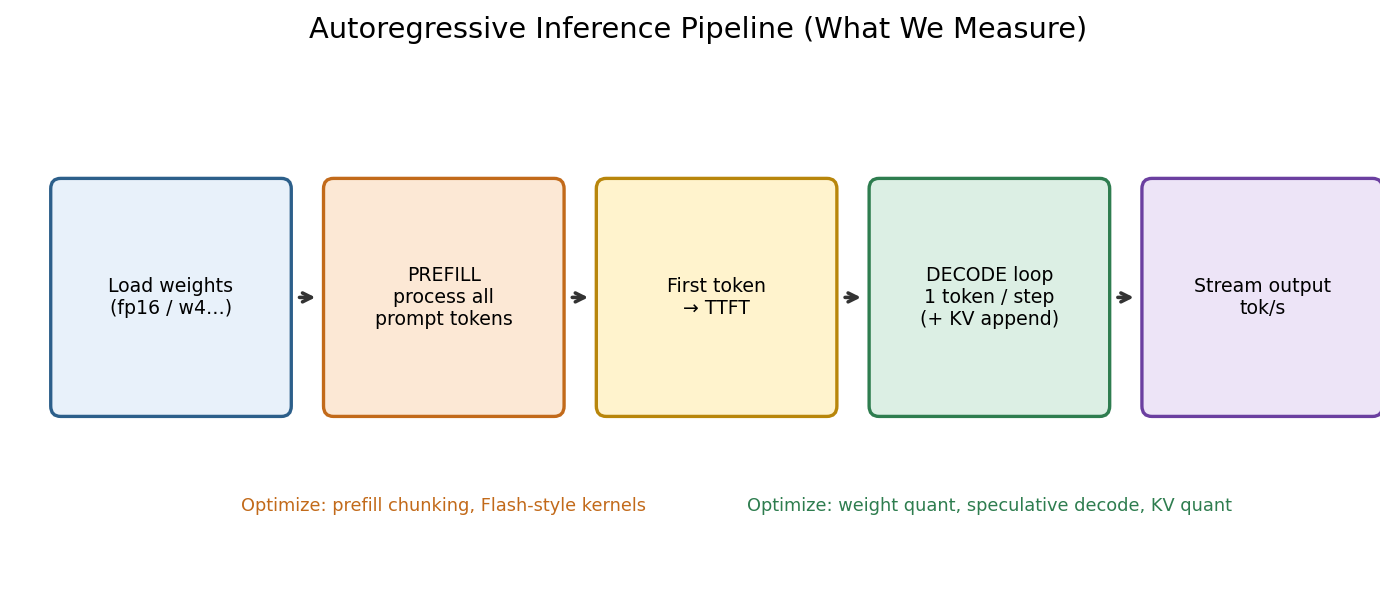
\includegraphics[width=0.98\linewidth]{figures/inference_pipeline.png}
  \caption{Single-request inference pipeline: load weights, prefill the prompt (TTFT), then autoregressive decode (tokens/s). Peak memory is a property of the whole run---the quantity everyday devices actually run out of.}
  \label{fig:pipeline}
\end{figure}

\subsection{Memory budget}

Peak resident memory is
\begin{equation}
  M_{\mathrm{peak}} \approx M_{\mathrm{weights}} + M_{\mathrm{KV}} + M_{\mathrm{act}} + M_{\mathrm{overhead}},
  \label{eq:peak}
\end{equation}
with static weights
\begin{equation}
  M_{\mathrm{weights}} \approx \frac{N \cdot b_w}{8}
  \label{eq:weights}
\end{equation}
for \(N\) parameters at \(b_w\) bits, and a KV cache
\begin{equation}
  M_{\mathrm{KV}} \approx 2\, L\, H_{\mathrm{kv}}\, T\, D\, \frac{b_{\mathrm{kv}}}{8}
  \label{eq:kv}
\end{equation}
for \(L\) layers, \(H_{\mathrm{kv}}\) key/value heads, head dimension \(D\), sequence length \(T\), and \(b_{\mathrm{kv}}\) bits per cached element~\citep{pope2022efficiently,ainslie2023gqa}. The factor of two is the pair \((K,V)\). Grouped-query and multi-query attention reduce \(H_{\mathrm{kv}}\) relative to query heads~\citep{shazeer2019mqa,ainslie2023gqa}. \(M_{\mathrm{overhead}}\) includes the framework, allocator fragmentation, and---critically on everyday devices---whatever the OS and apps already hold.

For a Llama-class 8B model, \(b_w = 16\) costs \(\approx 16\)\,GB of weights. At \(b_w = 4\) the same term is \(\approx 4\)\,GB. For \(L=32\), \(H_{\mathrm{kv}}=8\), \(D=128\), \(T=640\), FP16 KV is \(\approx 84\)\,MB; 4-bit KV is \(\approx 21\)\,MB. At \(T=4096\), FP16 KV is \(\approx 536\)\,MB. Weights set the \emph{floor}; KV sets the \emph{slope} in \(T\). Short-chat benches are weight-dominated and will lie about KV optimizations (Section~\ref{sec:kv}).

\subsection{Roofline view of decode}

When a decode step is memory-bandwidth bound~\citep{williams2009roofline},
\begin{equation}
  \mathrm{tok/s} \approx \frac{B_{\mathrm{mem}}}{B_{\mathrm{token}}},
  \label{eq:roofline}
\end{equation}
where \(B_{\mathrm{mem}}\) is sustained DRAM (or HBM) bandwidth and \(B_{\mathrm{token}}\) is bytes moved per generated token---dominated by reading the weights. Reducing \(b_w\) therefore raises tokens/s \emph{and} lowers \(M_{\mathrm{weights}}\). On a laptop this is why 4-bit is not only a fit trick: Llama~3.1~8B on an M3 moves from 5.8 to 20.5 tokens/s when \(b_w: 16 \to 4\), close to the byte-ratio prediction after kernel overheads.

Prefill can be much more compute- or attention-IO-bound as \(T_p\) grows. The same 4-bit checkpoint that streams well can still post a 15\,s TTFT at \(T_p=2048\).

\subsection{Unified memory versus discrete GPUs}

On a discrete GPU, weights live in HBM; the host CPU has a separate DRAM pool; PCIe is an explicit copy path. On Apple Silicon, CPU, GPU, and Neural Engine share one unified DRAM pool~\citep{apple2020silicon,mlx2023} (Figure~\ref{fig:um}). There is no host--device copy in the CUDA sense, and also \emph{no private VRAM ceiling}. Local 8B inference on a 24\,GB Mac is a packing problem first and a kernel problem second.

\begin{figure}[t]
  \centering
  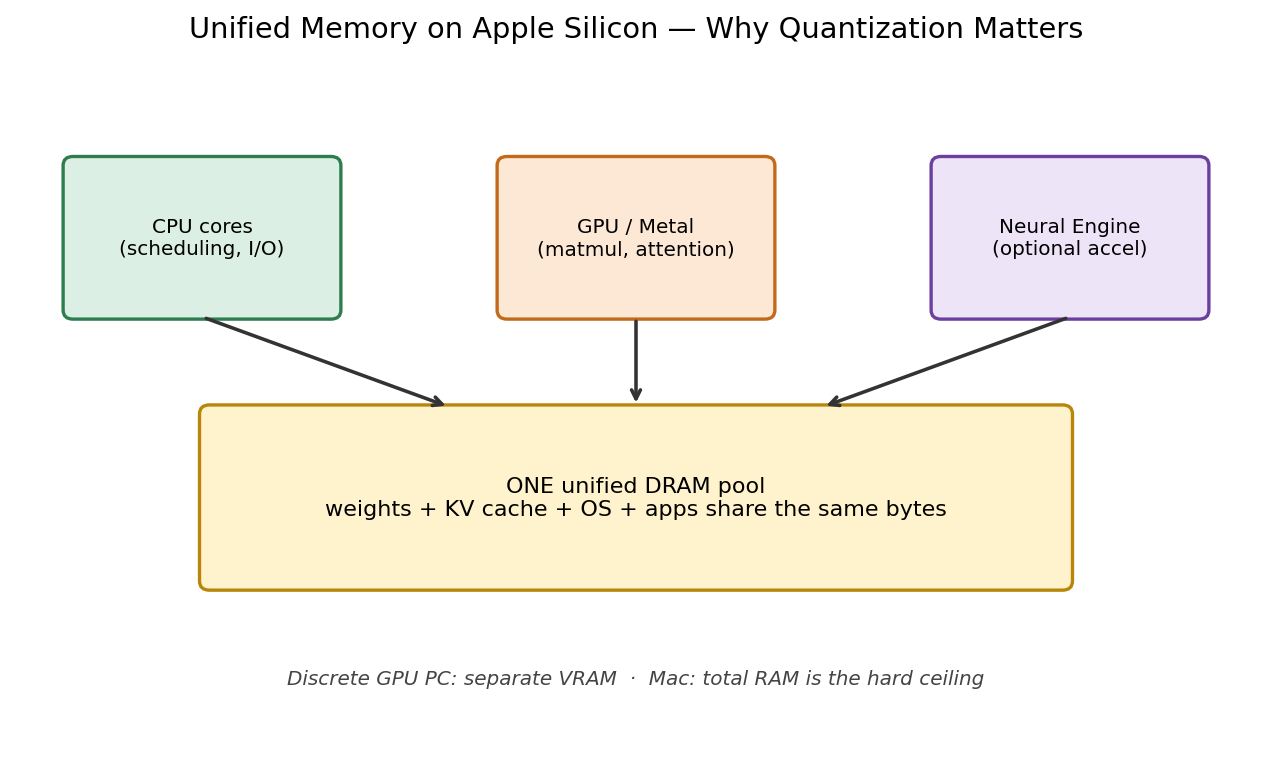
\includegraphics[width=0.92\linewidth]{figures/unified_memory.png}
  \caption{Unified memory on Apple Silicon: weights, KV cache, activations, and the operating system share one DRAM pool. Capacity planning \emph{is} the first optimization on everyday devices.}
  \label{fig:um}
\end{figure}

\subsection{Quality as a constraint, not a metric to maximize in this paper}

We do not claim that 4-bit matches FP16 on every reasoning bench. GPTQ/AWQ-class 4-bit is widely treated as the practical default for local chat and coding~\citep{frantar2022gptq,lin2023awq}; 2-bit and naive 3-bit remain research-to-product. A responsible local stack uses 4-bit as the daily driver and keeps a W8/FP16 checkpoint for eval nights (Section~\ref{sec:decision}).

\section{A bottleneck-first taxonomy}
\label{sec:taxonomy}

Table~\ref{tab:taxonomy} organizes techniques by the bottleneck they attack. Families are complementary: weight bits do not replace KV paging; speculative decoding does not shrink the checkpoint. On everyday devices the \emph{order} is not optional.

\begin{table*}[t]
  \centering
  \small
  \caption{Taxonomy of LLM inference optimizations. ``Daily-driver rank'' is how early a solo user on a 16--24\,GB machine should reach for the family.}
  \label{tab:taxonomy}
  \begin{tabularx}{\textwidth}{@{}>{\raggedright\arraybackslash}p{2.2cm}X>{\raggedright\arraybackslash}p{2.4cm}>{\raggedright\arraybackslash}p{1.6cm}@{}}
    \toprule
    Family & Representative methods & Bottleneck & Daily rank \\
    \midrule
    Weight / activation compression & FP16/BF16, INT8/4/2, GPTQ, AWQ, SmoothQuant, QuaRot, pruning, distillation & Capacity + decode bandwidth & 1st \\
    Architecture \& size & 0.5B--9B ladder, Phi/OpenELM/MobileLLM, MoE, long-context variants & Quality vs.\ fit & 1st \\
    KV cache \& context & KV quant, GQA/MQA, PagedAttention, prefix cache, H2O, StreamingLLM, SnapKV & Capacity slope in \(T\) & 2nd \\
    Attention \& prefill & FlashAttention, chunked prefill, MInference, sparse/local attn, RoPE/YaRN & Prefill compute / IO & 3rd \\
    Decode algorithms & Speculative decoding, Medusa, EAGLE, SpecInfer, graphs & Sequential decode & 4th \\
    Compilation \& runtimes & MLX, llama.cpp, MLC, ExecuTorch, \texttt{compile}, offload, mmap & Kernel efficiency & 4th \\
    Application-level & RAG sizing, prompt cache, constrained decoding, early exit & Tokens billed / prefilled & always \\
    Batching \& scheduling & Continuous batching, SLOs, disaggregated PD & Multi-request utilization & late \\
    Parallelism & Tensor, pipeline, expert, data parallel & Multi-device fit/latency & late \\
    Adapters & LoRA / QLoRA, multi-LoRA & Extra matmuls + RAM & as needed \\
    \bottomrule
  \end{tabularx}
\end{table*}

A useful stacking order for \emph{single-stream} local inference is: (1)~choose a model that can fit; (2)~quantize weights until there is OS headroom; (3)~quantize or page KV if context grows; (4)~tune prefill and \emph{shorten the prompt} if TTFT hurts; (5)~add speculation if decode still lags and RAM remains; (6)~only then change runtime or hardware. Multi-tenant serving inverts the last steps: paging and continuous batching become mandatory before exotic decode algorithms. Figure~\ref{fig:funnel} sketches the local funnel.

\begin{figure}[t]
  \centering
  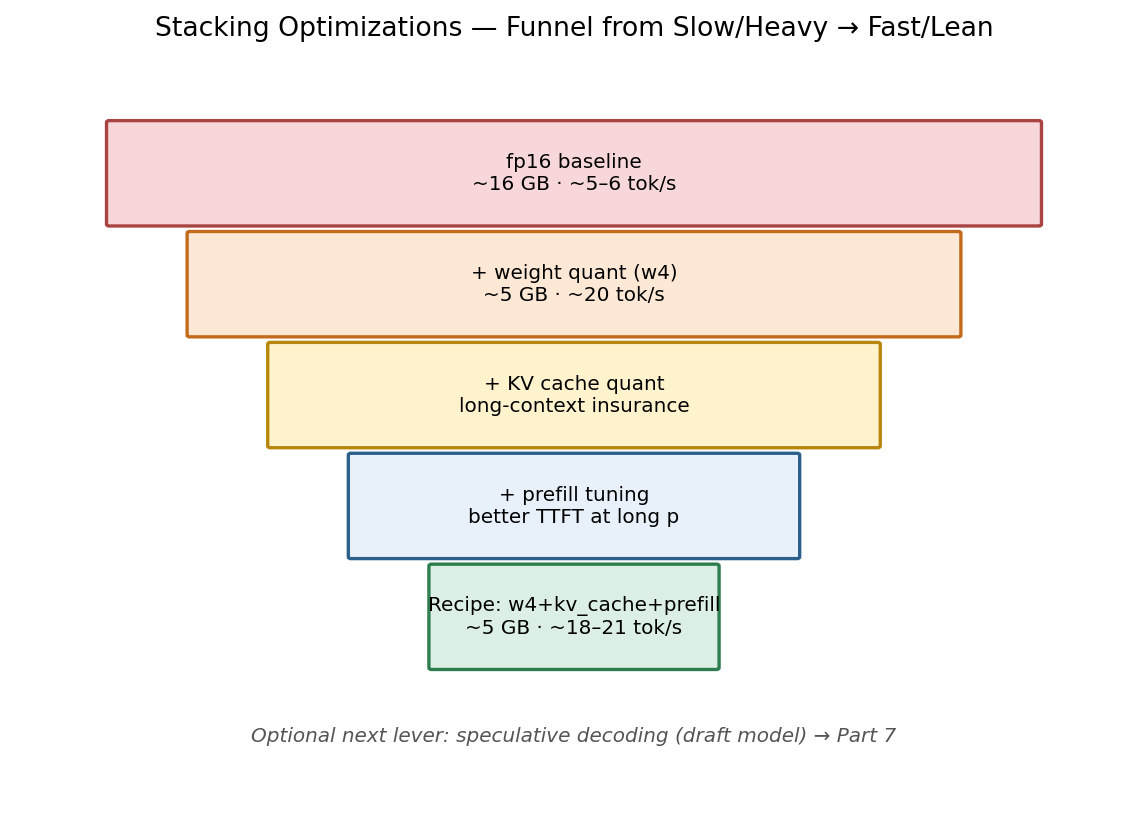
\includegraphics[width=0.98\linewidth]{figures/optimization_funnel.png}
  \caption{Local optimization funnel: weight bits shrink the floor, KV quantization insures growth in \(T\), prefill tuning attacks TTFT, and the daily recipe is the combination that survives the RAM budget \emph{with the rest of the computer still running}.}
  \label{fig:funnel}
\end{figure}

\section{Weight and activation compression}
\label{sec:weights}

\subsection{Affine quantization}

Affine quantization~\citep{jacob2018quantization} maps a real weight \(x\) to a \(b\)-bit integer code
\begin{equation}
  q = \mathrm{clip}\!\left(\mathrm{round}\!\left(\tfrac{x}{s}+z\right),\, 0,\, 2^{b}-1\right),
  \qquad
  \hat{x} = s\,(q-z),
\end{equation}
with scale \(s\) and zero-point \(z\), typically shared by a group of \(G\) weights (e.g.\ 64 or 128). Group-wise scales keep dynamic range honest when a tensor has outliers. At inference, kernels dequantize on the fly or compute in low precision so a full FP16 copy is never materialized. GPTQ was motivated by 175B-class models that could not fit on a single GPU~\citep{frantar2022gptq}; the same math now makes 8B models comfortable on a laptop---an inversion of the original constraint that is exactly the everyday-device story.

\subsection{Post-training methods for LLMs}

\textbf{GPTQ}~\citep{frantar2022gptq} quantizes weights column-by-column, using a Hessian-aware update so remaining weights compensate for rounding error. \textbf{AWQ}~\citep{lin2023awq} identifies activation-salient channels and protects them so aggressive 4-bit quantization does not destroy the directions the network actually uses. \textbf{LLM.int8()}~\citep{dettmers2022llmint8} keeps outlier features in higher precision during 8-bit matmul. \textbf{SmoothQuant}~\citep{xiao2023smoothquant} migrates quantization difficulty from activations into weights, enabling W8A8-style pipelines. \textbf{OmniQuant}~\citep{shao2024omniquant} learns quantization parameters. Rotation / incoherence methods---QuaRot~\citep{ashkboos2024quarot}, SpinQuant~\citep{che2024spinquant}, QuIP\#~\citep{tseng2024quip}---make weights easier to quantize by changing basis. Additive residual codebooks (AQLM~\citep{egiazarian2024aqlm}) and sparse-quantized hybrids (SpQR~\citep{frantar2023spqr}, SqueezeLLM~\citep{kim2023squeezellm}) isolate a tiny high-precision outlier set. QServe~\citep{lin2024qserve} pushes a W4A8KV4 co-design into a serving engine.

In deployed local stacks, practitioners usually \emph{load} a pre-quantized checkpoint (GPTQ/AWQ/GGUF/MLX-community) rather than calibrating at serve time. Bit width \(b_w \in \{16,8,4,2\}\) is then a first-class serving knob. Empirically, \textbf{4-bit is the default sweet spot on unified-memory laptops}: 8-bit still spends too much DRAM for a daily driver; 2-bit frequently shows quality cliffs (Section~\ref{sec:empirical}).

\subsection{Activation quantization, mixed precision, pruning, distillation}

Activation quantization (W8A8, W4A8) matters when GEMM is compute-bound or when activation RAM dominates---more common in prefill and large-batch serving than in single-stream decode. Mixed precision (AMP) keeps accumulators in FP32 while storing weights in FP16/BF16; it is the default, not an extra flag, in most GPU stacks.

Pruning~\citep{han2015deep,frantar2023sparsegpt,ma2023llmpruner} removes weights. Unstructured sparsity needs specialized kernels to beat dense 4-bit GEMM on a laptop; structured (channel/head) pruning is easier to serve but harder to keep accurate. Knowledge distillation~\citep{hinton2015distilling,sanh2019distilbert} produces a smaller student: it is a \emph{different model}, not a runtime switch, but it is often the highest-leverage ``optimization'' if a 1--3B student meets the product bar---the Phi/TinyLlama/OpenELM bet~\citep{abdin2024phi3,zhang2024tinyllama,mehta2024openelm}.

\section{KV cache and context memory}
\label{sec:kv}

\subsection{Why the cache exists}

Scaled dot-product attention~\citep{vaswani2017attention} is
\begin{equation}
  \mathrm{Attention}(Q,K,V)=\mathrm{softmax}\!\left(\frac{QK^{\top}}{\sqrt{d_h}}\right)V.
\end{equation}
Recomputing \(K,V\) for the entire history at every decode step would repeat \(O(T)\) work per token. Caching per-layer \(K\) and \(V\) makes decode \(O(1)\) cache appends plus attention against the stored history. Equation~\eqref{eq:kv} then grows linearly in \(T\).

On a 24\,GB machine with 4-bit 8B weights ($\approx 5$\,GB), the cache is a rounding error at \(T=640\) and a second-class citizen that becomes first-class at long RAG, multi-turn agents, or (in servers) many concurrent sequences. Short-chat A/B tests that ``prove KV quant does nothing'' are measuring the wrong \(T\).

\subsection{Fewer KV heads}

Multi-query attention~\citep{shazeer2019mqa} shares one KV head across query heads. Grouped-query attention~\citep{ainslie2023gqa} interpolates, with \(H_{\mathrm{kv}} \ll H_q\). This is an \emph{architectural} reduction of \(M_{\mathrm{KV}}\) and of cache bandwidth. It explains why two 7B models can have very different long-context RAM slopes, and why Llama-3-class GQA is so friendly to laptops.

\subsection{Quantizing the cache}

KV quantization stores cached \(K,V\) at \(b_{\mathrm{kv}} < 16\) (commonly 8, 4, or even 2). It is independent of \(b_w\). KIVI~\citep{liu2024kivi} uses asymmetric 2-bit KV without fine-tuning. KVQuant~\citep{hooper2024kvquant} targets million-token contexts. Quality impact is usually smaller than aggressive weight quantization because each decode step only \emph{reads} the cache rather than using it as the model's entire knowledge. On-device, enable it as insurance once 4-bit weights have created headroom---especially on 16\,GB machines with less slack for RAG.

\subsection{Paging, prefix reuse, eviction, and sparsity}

\textbf{PagedAttention}~\citep{kwon2023vllm} stores KV in non-contiguous blocks so a serving engine can pack many sequences (Figure~\ref{fig:paged}). A laptop running one chat does not need a pager; a laptop running a local multi-user \texttt{llama-server} does. \textbf{Prefix / prompt caching} reuses KV for a repeated system prompt or RAG template: the first request pays prefill, later requests skip it. This is one of the highest-ROI everyday-device tricks and the local analogue of a provider's prompt cache.

\textbf{Eviction} drops tokens believed unimportant: H\(_2\)O keeps heavy hitters~\citep{zhang2023h2o}; StreamingLLM keeps an attention sink plus a sliding window~\citep{xiao2024streamingllm}; SnapKV~\citep{li2024snapkv} and Quest~\citep{tang2024quest} select what to keep given the query; DuoAttention~\citep{xiao2024duoattention} splits retrieval and streaming heads. Sliding-window attention (Mistral-style) bounds KV by construction~\citep{mistral2023}. These trade exact long-range attention for a bounded RAM envelope---exactly the phone/laptop deal.

\begin{figure}[t]
  \centering
  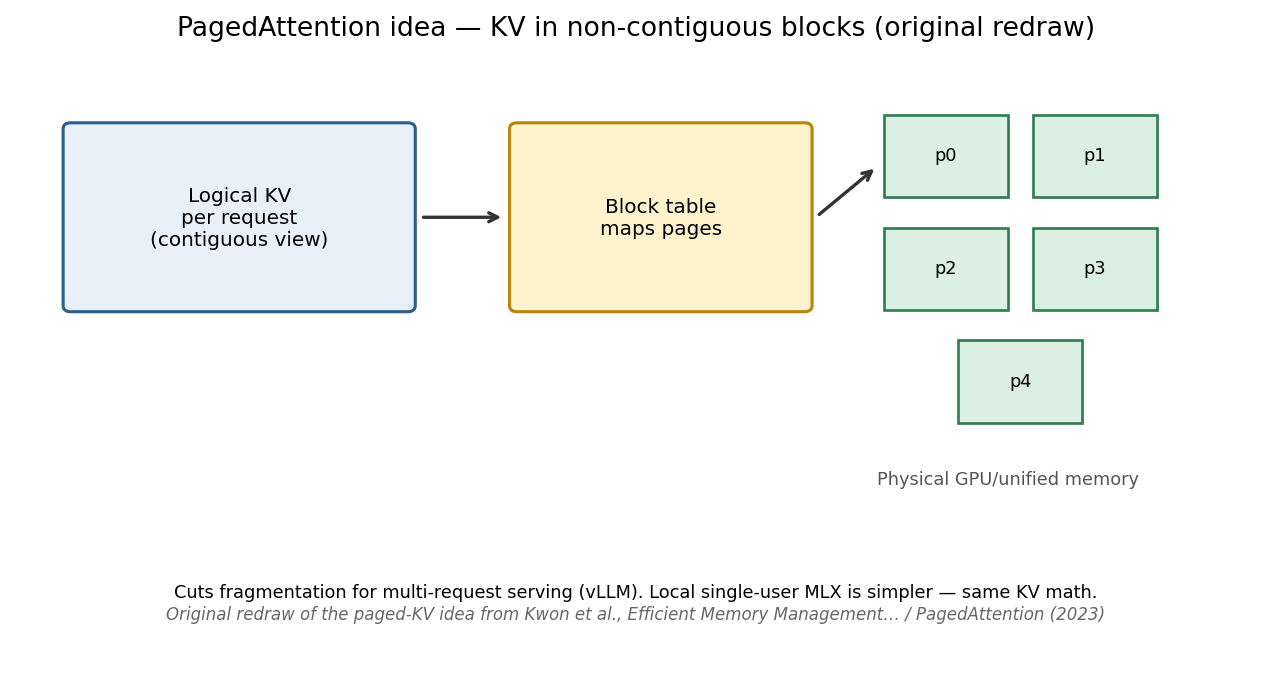
\includegraphics[width=0.92\linewidth]{figures/paged_attention.png}
  \caption{Paged KV (redraw after Kwon et al., 2023). Multi-user serving pages the cache; a daily-driver laptop is the single-tenant cousin of the same memory problem.}
  \label{fig:paged}
\end{figure}

\section{Attention kernels and prefill}
\label{sec:prefill}

Naive attention materializes \(S \in \mathbb{R}^{n \times n}\) per head. At \(n=2048\) and FP16 that is already \(\approx 8\)\,MB per head per layer. FlashAttention~\citep{dao2022flashattention} tiles \(Q,K,V\) through on-chip SRAM, uses an online softmax~\citep{milakov2018online}, and never writes the full score matrix to HBM. FlashAttention-2/3 improve parallelism and low-precision paths~\citep{dao2023flashattention2,dao2024flashattention3}. On Apple Silicon, MLX implements tiled Metal attention internally; user code rarely toggles a ``Flash'' flag. The user-visible leftover knob is often \textbf{chunked prefill} (prefill step size \(C\))~\citep{agrawal2023sarathipreprint,agrawal2024sarathi}: smaller \(C\) lowers peak activation memory; larger \(C\) often lowers TTFT when the device is under-occupied.

Long-prompt prefill is where everyday RAG dies. MInference~\citep{jiang2024minference} sparsifies prefill attention dynamically. Sparse and local attention~\citep{child2019sparse,beltagy2020longformer} reduce the \(O(n^2)\) term by restricting the pattern. State-space models~\citep{gu2023mamba} change the architecture. Rotary embeddings~\citep{su2024rope} and YaRN~\citep{peng2023yarn} extend usable context without a full pretrain; they do not by themselves reduce \(M_{\mathrm{KV}}\).

On a MacBook, the first prefill optimization is still application-level: retrieve fewer chunks (Section~\ref{sec:app}). The second is prefix cache. The third is kernels and \(C\).

\section{Decode-time algorithms}
\label{sec:decode}

\subsection{Speculative decoding}

Baseline decode costs \(\approx T_g \cdot \tau_t\) where \(\tau_t\) is one target-model forward. Speculative decoding~\citep{leviathan2023speculative,chen2023speculative} uses a cheap draft to propose \(k\) tokens; the target verifies them in one parallel forward and accepts a prefix of length \(m \le k\) under a rejection-sampling rule that preserves the target distribution (Figure~\ref{fig:spec}).

Let \(\alpha\) be the per-token acceptance probability. Wall-clock speedup requires \(\tau_d \ll \tau_t\) and high \(\alpha\). If the draft is a poor match, one still pays \(\tau_d + \tau_{\mathrm{verify}}\) and can \emph{lose} throughput---we measure this on Llama~3.1~8B (Section~\ref{sec:empirical}). Medusa~\citep{cai2024medusa} attaches extra heads to the target instead of a second model (attractive on phones where loading two graphs hurts). EAGLE~\citep{li2024eagle} drafts at the feature level. SpecInfer~\citep{miao2024specinfer} uses token trees. Lookahead and blockwise methods~\citep{chen2021lookahead,stern2018blockwise,spector2023rest} and Jacobi-style parallel decoding~\citep{santilli2023jacobidecoding} are related. Deja Vu~\citep{liu2024dejavu} skips compute via contextual sparsity.

On everyday devices speculation is a \emph{fourth} lever: it needs the RAM that 4-bit weights just freed, a tokenizer-compatible draft (0.5B--1B class), and a kill-switch when \(\alpha\) drops. CUDA graphs / Metal capture replay a static decode graph and help small-batch latency; they are complementary, not a substitute for bits.

\begin{figure}[t]
  \centering
  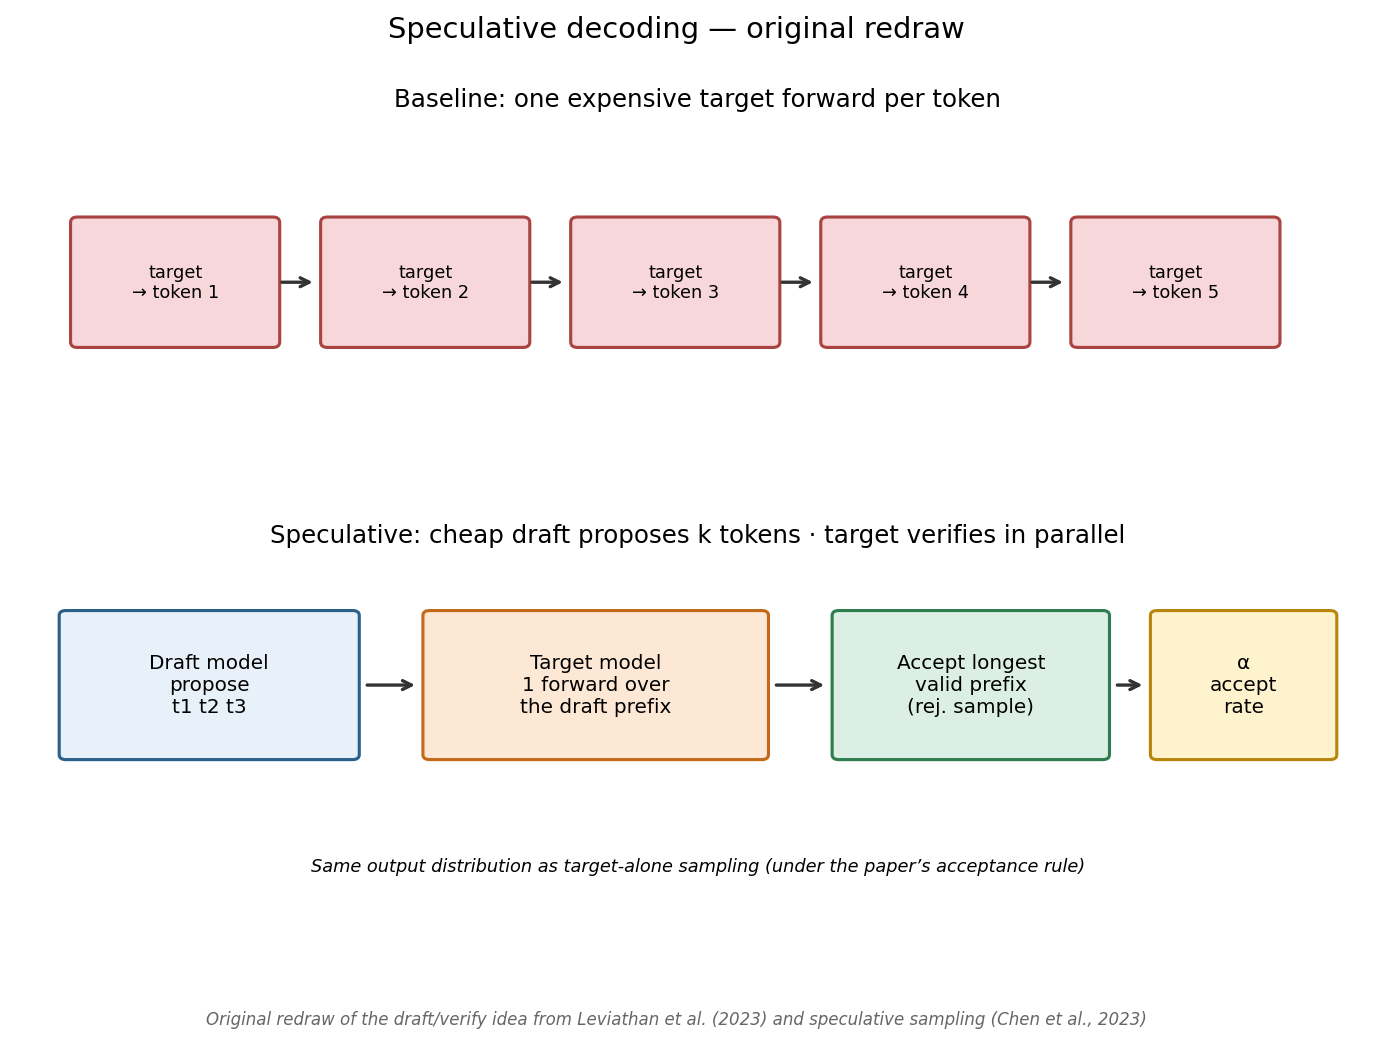
\includegraphics[width=0.92\linewidth]{figures/speculative.png}
  \caption{Speculative decoding (redraw after Leviathan et al.\ and Chen et al.). Speedup tracks acceptance \(\alpha\) and draft cost, not merely the presence of a draft---critical on memory-tight laptops.}
  \label{fig:spec}
\end{figure}

\section{Batching, scheduling, and disaggregation}
\label{sec:serving}

Local \texttt{generate()} loops are single-stream. Production serving is not. We include this family because (i)~the same human may later run \texttt{llama-server} for a household, and (ii)~papers in this family invented paging and chunked prefill that local stacks now expose as flags.

\textbf{Static batching} waits to fill a batch of size \(B\). \textbf{Continuous batching} (iteration-level scheduling)~\citep{yu2022orca,kwon2023vllm} mixes prefill of new requests with decode of in-flight ones. \textbf{Chunked prefill} in Sarathi-Serve~\citep{agrawal2024sarathi} piggybacks decode tokens alongside partial prefills. \textbf{Disaggregated prefill/decode}~\citep{patel2024splitwise,aminabadi2024distserve} places the two phases on different pools. SGLang~\citep{zheng2024sglang} adds a radix cache and structured generation. Request scheduling adds SLOs and preemption.

On a daily-driver laptop with one user, continuous batching does almost nothing. On a Mac mini serving a family, it suddenly does. The mistake is cargo-culting vLLM flags before the model fits beside Safari.

\section{Parallelism}
\label{sec:parallel}

When one device cannot hold the model, inference reuses training sharding: tensor parallel~\citep{shoeybi2019megatron,narayanan2021efficient}, pipeline parallel~\citep{huang2019gpipe}, expert parallel for MoE~\citep{fedus2022switch,lepikhin2021gshard,jiang2024mixtral,yi2023edgemoe}, and data parallel for large batches. Consumer Macs almost never expose multi-GPU tensor parallel for LLMs; the relevant decision is ``does this dense 70B fit in unified memory at 4-bit?'' (usually no on 24\,GB; sometimes yes on 128\,GB Ultra). A single consumer NVIDIA GPU plus CPU offload~\citep{sheng2023flexgen,song2024powerinfer,alizadeh2024llm} is the PC analogue. EdgeMoE~\citep{yi2023edgemoe} specifically targets on-device MoE.

\section{Architecture and model-size choices}
\label{sec:arch}

The highest-leverage ``optimization'' on a small machine is sometimes a smaller model. Memory~\eqref{eq:weights} and bandwidth-bound decode~\eqref{eq:roofline} both scale with \(N\). A dense 0.5B 4-bit model and a dense 8B 4-bit model can differ by an order of magnitude in tokens/s on the same laptop (Section~\ref{sec:empirical}). Phi-3~\citep{abdin2024phi3}, TinyLlama~\citep{zhang2024tinyllama}, OpenELM~\citep{mehta2024openelm}, MobileLLM~\citep{liu2024mobilellm}, Gemma~2 2B~\citep{team2024gemma2}, and Llama~3.2 1B/3B exist because of that curve. Mixture-of-experts~\citep{jiang2024mixtral,liu2024deepseek} offers more total parameters at a smaller active-FLOP budget, at the cost of a larger memory floor---painful on 16\,GB, interesting on 64\,GB. Long-context variants inflate \(T\) in~\eqref{eq:kv} and prefill cost. Instruction-tuned versus base checkpoints should be held fixed in systems benchmarks; they are not speed knobs.

\section{Adapters}
\label{sec:lora}

LoRA~\citep{hu2022lora} injects low-rank updates \(BA\) into frozen weights. QLoRA~\citep{dettmers2023qlora} fine-tunes those adapters on a quantized base---the reason a laptop can specialize an 8B model overnight. At inference, each adapter adds a small extra GEMM and RAM. Multi-LoRA serving swaps adapters per request; that is a server problem. For a single local user, one LoRA is usually noise compared with \(b_w\), and it is how ``my coding style'' becomes an on-device file rather than a cloud fine-tune.

\section{Compilation, kernels, and runtimes}
\label{sec:runtime}

Graph compilation (\texttt{torch.compile}, \texttt{mlx.compile}, XLA, TensorRT-LLM~\citep{nvidia2024trtllm}, MLC~\citep{mlcllm}) fuses ops and specializes shapes. Quantized matmul kernels determine whether 4-bit is actually faster than FP16 or merely smaller. CPU/disk offload~\citep{sheng2023flexgen,alizadeh2024llm} runs models that do not fit, at a large bandwidth penalty. Memory-mapping weights from SSD reduces cold-start RAM spikes.

Local runtimes illustrate that \emph{the same bit width is not the same system}:

\begin{itemize}[leftmargin=*,itemsep=2pt]
  \item \textbf{MLX / mlx-lm}~\citep{mlx2023,mlxlm2023}: Metal-native arrays, Hugging Face \texttt{mlx-community} checkpoints, Python harnesses---the path we measure.
  \item \textbf{llama.cpp / GGUF}~\citep{llamacpp,gguf}: C/C++, Metal/CUDA/CPU, community GGUF quants (Q4\_K\_M, Q8\_0, \ldots). The default engine behind much of local-LLM culture.
  \item \textbf{Ollama}~\citep{ollama}: distribution and UX over llama.cpp-class engines.
  \item \textbf{MLC LLM}~\citep{mlcllm}: TVM compilation across GPU/NPU/CPU.
  \item \textbf{ExecuTorch}~\citep{executorch}: mobile/edge PyTorch.
  \item \textbf{PowerInfer}~\citep{song2024powerinfer}: hot-neuron GPU + cold-neuron CPU on a consumer PC.
\end{itemize}

Fair comparison requires matched prompts, generation length, and a comparable quant \emph{tier} (FP16 vs.\ F16 GGUF; 4-bit MLX vs.\ Q4\_K\_M), not matched marketing names.

\section{Application-level inference}
\label{sec:app}

Not every latency problem belongs inside the model---especially on everyday devices, where the user controls the prompt.

Retrieval-augmented generation~\citep{lewis2020rag} can \emph{increase} TTFT by stuffing thousands of tokens into \(T_p\). The correct optimization is often ``retrieve less'' or ``rerank then truncate.'' Prefix caches (Section~\ref{sec:kv}) absorb repeated templates. Semantic prompt caches reuse prior completions. Constrained / structured decoding~\citep{willard2023outlines,zheng2024sglang} masks logits toward JSON or grammars; it adds CPU work per token. Early-exit and confidence stopping~\citep{schuster2022confident} cut \(T_g\). Nucleus and temperature~\citep{holtzman2020nucleus} are quality knobs with mild speed effects. Tool/function calling~\citep{alizadeh2024llmcompiler} is an application graph; on a laptop, serial tool loops dominate wall-clock more than GEMM.

The daily-driver heuristic: \textbf{every token you do not retrieve is a token you do not prefill.}

\section{Empirical study: daily-driver laptops}
\label{sec:empirical}

The taxonomy is only useful if the local, measurable subset is actually measured on the class of machine people use. We summarize a public harness\footnote{Companion repository: LLM-Inference. Isolated subprocesses, schema-versioned JSON, median of trials after one warmup.} that holds prompt length, generation length, and trial policy fixed, and varies one family at a time and then in combination.

\paragraph{Hardware.}
Mac M3 with \textbf{24\,GB} unified memory---the canonical daily-driver laptop in this study---and Mac M5 Max (workstation-class M-series). Same prompts, same token counts, same config labels.

\paragraph{Default shape.}
\(T_p=512\), \(T_g=128\), unless noted. Models are mlx-community checkpoints (Llama~3.1, Mistral, Qwen, Gemma, and related presets). Configurations: \texttt{fp16}, \texttt{w8}, \texttt{w4}, \texttt{w2}, with optional \texttt{+kv\_cache} (4-bit KV) and \texttt{+prefill} (\(\texttt{prefill\_step\_size}=2048\) vs.\ 512).

\subsection{Weight quantization dominates the floor}

On Mac M3, Llama~3.1~8B (Table~\ref{tab:bits}):

\begin{table}[t]
  \centering
  \small
  \caption{Llama~3.1~8B weight-bit sweep on Mac M3 (24\,GB), \(T_p=512\), \(T_g=128\).}
  \label{tab:bits}
  \begin{tabular}{@{}lcccc@{}}
    \toprule
    Config & Peak GB & TTFT (ms) & tok/s & vs fp16 \\
    \midrule
    fp16 & 16.33 & 2637 & 5.8 & \(1.0\times\) \\
    w8 & 8.96 & 2775 & 11.3 & \(1.9\times\) \\
    w4 & 5.06 & 2738 & 20.5 & \(3.5\times\) \\
    w2 & 3.11 & 2826 & 35.8 & \(6.2\times\) \\
    \bottomrule
  \end{tabular}
\end{table}

FP16 at 16.3\,GB on a 24\,GB machine is not a daily driver: the OS and a browser barely fit. 4-bit is the knee of the memory--speed Pareto (Figure~\ref{fig:pareto}): the laptop stays a laptop. 2-bit wins the leaderboard and is the first place quality complaints concentrate; we treat it as a last resort, not a silent default. Across 14 M3-feasible presets the same pattern holds: fewer bits raise tokens/s because decode is bandwidth-bound~\eqref{eq:roofline}.

\begin{figure}[t]
  \centering
  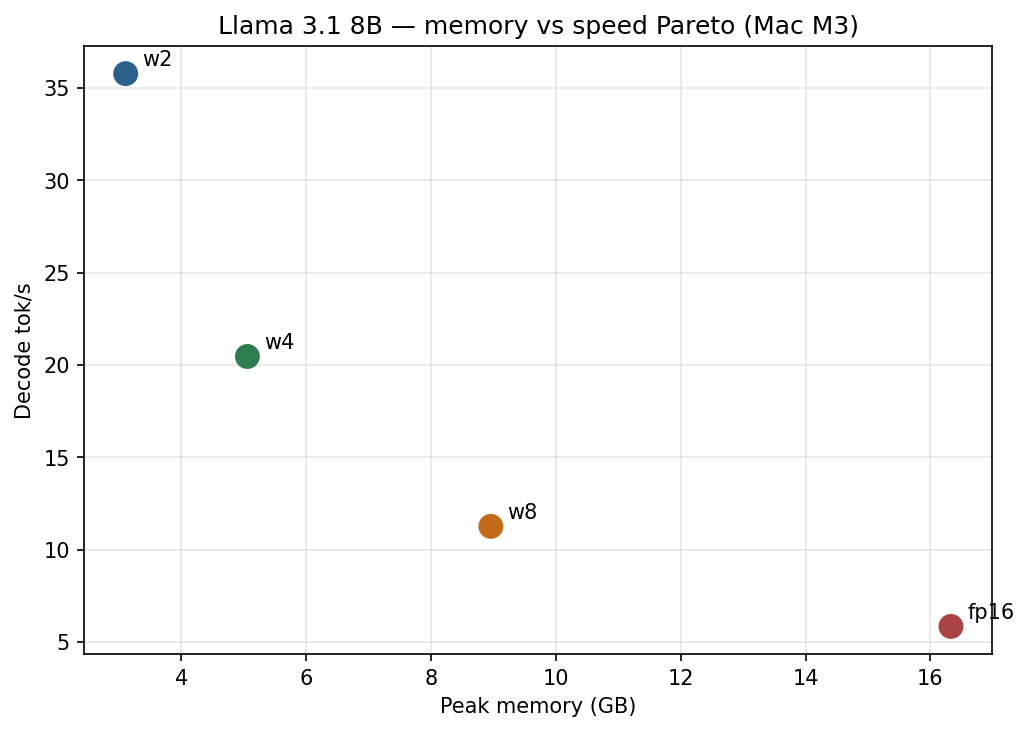
\includegraphics[width=0.98\linewidth]{figures/pareto.png}
  \caption{Memory--speed Pareto across weight bit-widths and models. Moving from FP16 to 4-bit is a joint win on both axes for bandwidth-bound decode---the difference between ``science fair'' and ``I leave this running all day.''}
  \label{fig:pareto}
\end{figure}

\subsection{Stacking KV quantization and prefill}

Table~\ref{tab:stack} is the capstone. Adding 4-bit KV and larger prefill chunks on top of 4-bit weights yields \textbf{5.06\,GB} and \textbf{19.9 tokens/s} for Llama~3.1~8B on M3 (\(\approx 3.55\times\) decode vs.\ FP16, \(\approx 31\%\) of FP16 memory). Mistral~7B moves from 3.6 to 16.0 tokens/s and 14.8 to 4.6\,GB (\(\approx 4.4\times\)). The \(\approx 11\)\,GB clawed back from Llama FP16 is enough to hold another 7--8B 4-bit model, or a fat RAG cache, \emph{or Chrome}.

\begin{table}[t]
  \centering
  \small
  \caption{Full stack on Mac M3 (24\,GB). Fully optimized \(=\) \texttt{w4+kv\_cache+prefill}.}
  \label{tab:stack}
  \begin{tabular}{@{}lccc@{}}
    \toprule
    Model / recipe & Peak GB & TTFT (ms) & tok/s \\
    \midrule
    Llama 3.1 8B, fp16 & 16.33 & 2689 & 5.6 \\
    Llama 3.1 8B, full stack & 5.06 & 2746 & 19.9 \\
    Mistral 7B, fp16 & 14.77 & 4350 & 3.6 \\
    Mistral 7B, full stack & 4.62 & 3954 & 16.0 \\
    \bottomrule
  \end{tabular}
\end{table}

TTFT barely moves on this \emph{short} prompt. That is expected: prefill's value shows up when \(T_p\) climbs. KV quantization's absolute gigabyte win is small at \(T=640\); it is insurance for long \(T\). On short chats, enabling KV+prefill on top of w4 can even cost a few tokens/s. Ship \texttt{w4+kv\_cache+prefill} as a \emph{product preset}; bench plain \texttt{w4} if you want peak short-chat speed.

At default \(T\), Llama~3.1~8B w4 vs.\ w4+KV on M3 is 20.7 vs.\ 20.4 tokens/s (about \(-1.5\%\)); Mistral and Qwen~2.5~7B similarly. The knob is not a dud---the benchmark is weight-dominated.

\subsection{The 16-config matrix on M5 Max}

Weight bits \(\times\) KV on/off \(\times\) prefill on/off is \(4\times 2\times 2 = 16\) configs. Table~\ref{tab:m5mat} (Llama~3.1~8B, M5 Max) shows the ladder: fp16 \(\approx 35\) tok/s at 16.5\,GB, w8 \(\approx 64\) at 9.0\,GB, w4 \(\approx 112\) at 5.1\,GB, w2 \(\approx 178\) at 3.3\,GB. KV and prefill barely change short-prompt decode. Mistral~7B on the same machine: fp16 \(\approx 37\) tok/s at 14.9\,GB \(\rightarrow\) optimized \(\approx 114\) tok/s at 4.7\,GB.

\begin{table}[t]
  \centering
  \small
  \caption{Selected cells of the Llama~3.1~8B matrix on Mac M5 Max (decode tok/s / peak GB).}
  \label{tab:m5mat}
  \begin{tabular}{@{}lcc@{}}
    \toprule
    Config & tok/s & Peak GB \\
    \midrule
    fp16 & 35.1 & 16.46 \\
    w8 & 63.6 & 8.97 \\
    w4 & 112.5 & 5.11 \\
    w4+kv+prefill & \(\approx 107\) & 5.11 \\
    w2 & 178.0 & 3.26 \\
    \bottomrule
  \end{tabular}
\end{table}

\begin{figure}[t]
  \centering
  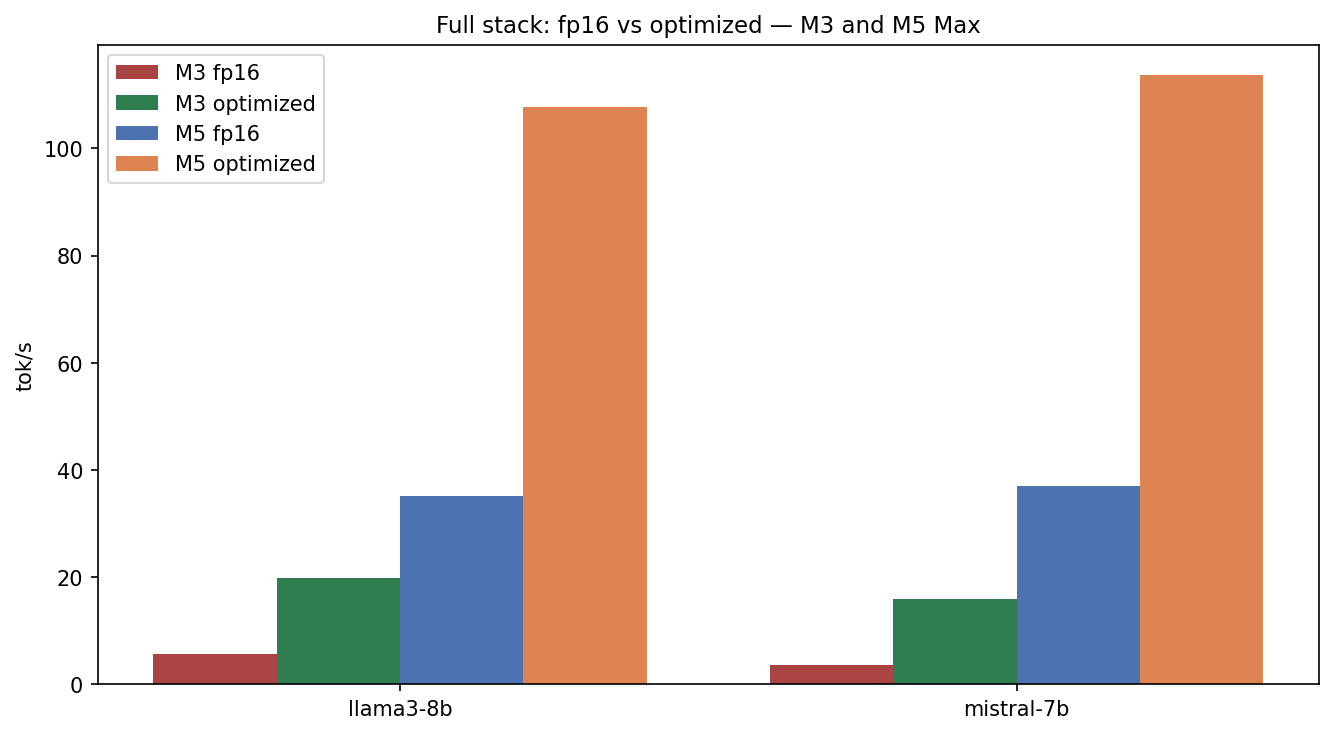
\includegraphics[width=0.98\linewidth]{figures/m3_m5_stack.png}
  \caption{Same software stack, two chips. Relative wins from leaving FP16 travel; absolute UX does not: \(\approx 20\) tok/s on M3 is usable chat, \(\approx 100+\) tok/s on M5 Max makes the UI the bottleneck.}
  \label{fig:m3m5}
\end{figure}

Relative stacking math is portable across M3 and M5. Absolute UX is not. Memory geometry is portable: \(\approx 5\)\,GB for an 8B w4 stack is the planning number on both. M5 makes ``FP16 for quality nights'' realistic (\(\approx 35\) tok/s); on M3, FP16 8B is a last resort.

\subsection{Model-size ladder}

Holding the recipe at 4-bit, M3 decode spans \textbf{238 tokens/s} at Qwen~2.5~0.5B (0.64\,GB) down to \textbf{20.6 tokens/s} at Llama~3.1~8B (5.06\,GB) and \textbf{15.4 tokens/s} at Gemma~2~9B (5.88\,GB)---about \(15\times\) from the tiny tier to the top of the ``real laptop'' tier before leaving single-digit billions of parameters (Figure~\ref{fig:ladder}). On M5 Max, Llama~8B 4-bit reaches \(\approx 112\) tokens/s and Gemma~27B 4-bit remains interactive at \(\approx 33\) tokens/s. Hardware bandwidth multiplies the same stack; it does not replace quantization on a 24\,GB machine. If you pick models by social-media vibes alone you will either swap a 70B to death or run a 0.5B and wonder why reasoning collapsed.

\begin{figure}[t]
  \centering
  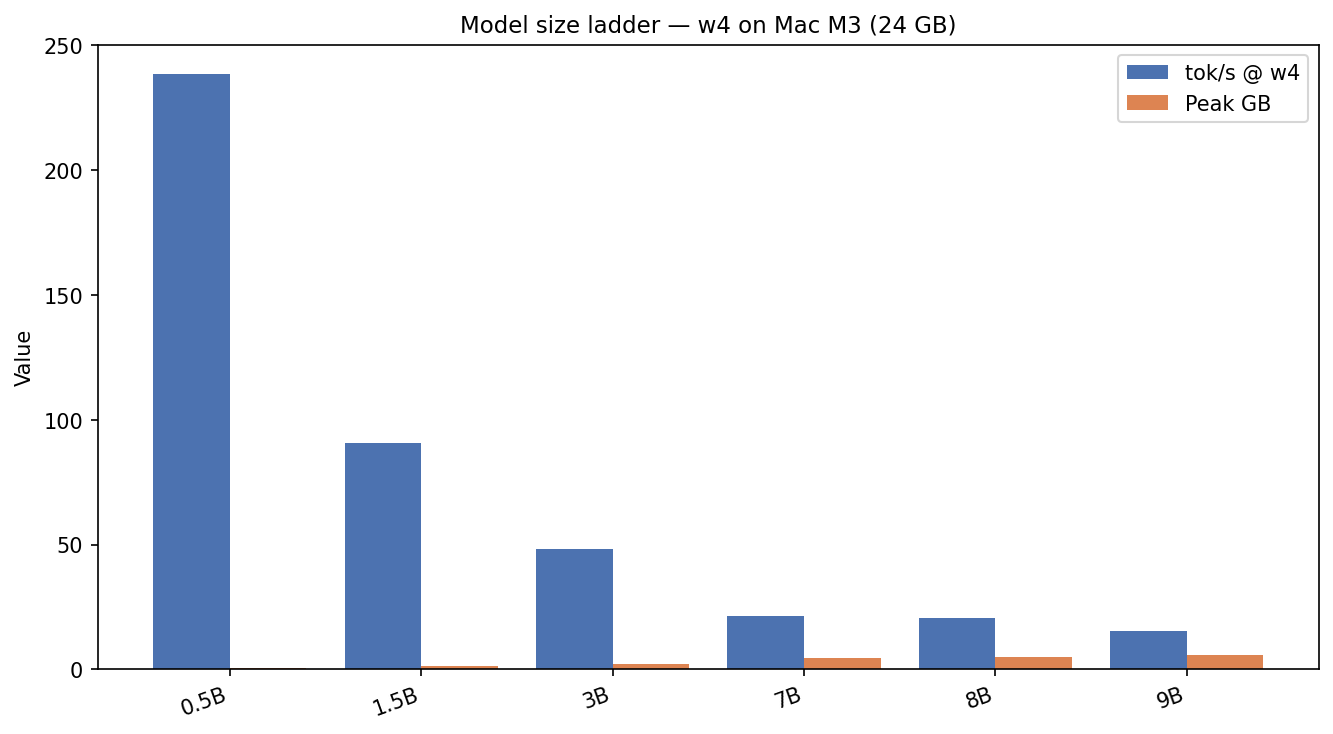
\includegraphics[width=0.98\linewidth]{figures/model_ladder.png}
  \caption{Dense 4-bit model ladder on Apple Silicon. Size is an inference optimization: quality, memory, and tokens/s move together.}
  \label{fig:ladder}
\end{figure}

\subsection{Speculative decoding is not unconditionally faster}

With a small 4-bit draft, Qwen~2.5~7B on M3 goes from 15.9 to \textbf{28.3 tokens/s} (\(1.78\times\)) at acceptance \(\alpha=74.2\%\), adding only \(\approx 0.3\)\,GB---possible only because 4-bit weights already freed RAM. The same pair on M5 Max goes from 122 to 170.3 tokens/s at the same \(\alpha\). Llama~3.1~8B on M5 Max is a negative result: 113.5 \(\rightarrow\) 109.7 tokens/s at \(\alpha=58.6\%\). Speculation should be reported with \(\alpha\) and a baseline, never as a guaranteed badge on a laptop preset.

\subsection{Context, RAG, and prefix cache}

Prefill TTFT grows steeply with \(T_p\) (Figure~\ref{fig:ttft}). On M3 with Llama~3.1~8B w4: \(T_p=256\) \(\rightarrow\) 2.4\,s TTFT; \(T_p=512\) \(\rightarrow\) \(\approx 3.1\)\,s; \(T_p=1024\) \(\rightarrow\) 5.8\,s; \(T_p=2048\) \(\rightarrow\) \(\approx 15.4\)\,s. A \texttt{rag\_agent} workload with \(T_p=4096\) records TTFT \(\approx 31.1\)\,s on M3 versus \(\approx 1.5\)\,s on M5 Max. That is a product failure on the smaller chip even when decode tokens/s look acceptable. Prefix KV cache converts a repeated system prompt from a prefill into a cache hit. Generation-length sweeps confirm Equation~\eqref{eq:kv}: decode tokens/s decay slowly as attention over the cache grows; peak memory tracks \(T\).

\begin{figure}[t]
  \centering
  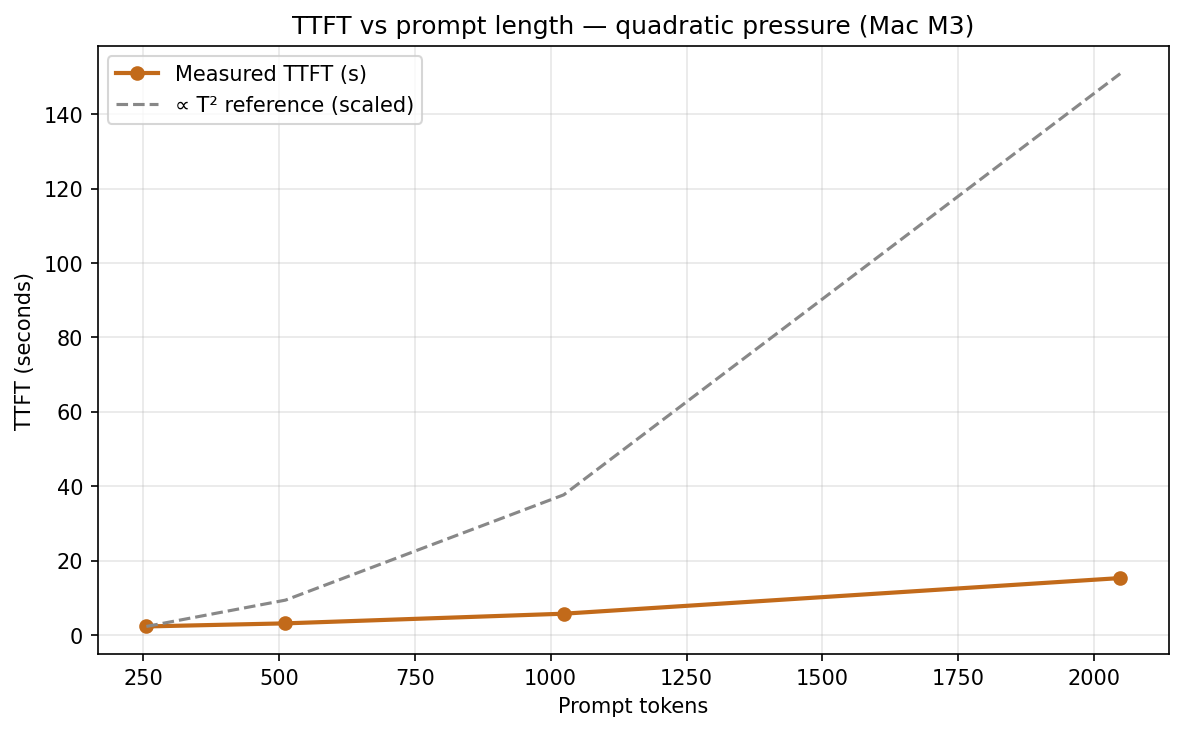
\includegraphics[width=0.98\linewidth]{figures/ttft_curve.png}
  \caption{TTFT versus prompt length. Local RAG dies in prefill, not in the tokens/s column. Everyday-device UX is a prefill SLO.}
  \label{fig:ttft}
\end{figure}

\subsection{Runtimes}

MLX and llama.cpp implement overlapping quant tiers on the same Metal GPU. In matched-tier comparisons (FP16 vs.\ F16 GGUF; 4-bit vs.\ Q4\_K\_M), neither engine universally wins; kernel quality, thread pinning, and quant layout dominate. Ollama is a packaging layer. The practical rule: pick the runtime that exposes the lever you need (MLX for Python sweeps; llama.cpp for portable GGUF and CPU fallback), then freeze it while you sweep \(b_w\) and \(T\).

\section{Recipes and a decision procedure}
\label{sec:decision}

\subsection{Steal these presets}

\paragraph{Daily driver --- 24\,GB laptop (M3-class).}
Config \texttt{w4+kv\_cache+prefill}; models Llama~8B / Mistral~7B / Qwen~7B; expect \(\approx 4.6\)--\(5.1\)\,GB peak and \(\approx 16\)--\(21\) tokens/s. Do not use FP16 8B as the always-on default.

\paragraph{16\,GB laptop or large phone.}
Stay at 1B--3B @ 4-bit as the assistant (Phi-3-class, Llama~3.2~3B, Qwen~2.5~3B); 7--8B @ 4-bit only with discipline and KV quant on. Skip FP16 7B+ entirely.

\paragraph{Quality / eval night, same 24\,GB machine.}
W8, or FP16 with other apps closed. Better fidelity, half or full memory pain. Not the always-on assistant.

\paragraph{M5 Max / 64\,GB+ desk.}
Chat default still \texttt{w4+kv\_cache+prefill} (\(\approx 107\) tok/s Llama~8B). Short-chat peak: plain w4 (\(\approx 112\)). FP16 8B is now an interactive eval mode (\(\approx 35\) tok/s). 27B @ 4-bit is usable. 70B still wants quantization and a sober look at \(T\).

\paragraph{Phone / NPU.}
Ship a 1--3B 4-bit (or vendor foundation model~\citep{gunter2024apple,abdin2024phi3}); treat 7B as optional on flagship RAM only; prefer Medusa-style heads over a second draft graph if memory is the wall.

\subsection{Symptom \(\rightarrow\) first lever}

Table~\ref{tab:decision} maps the failure the user actually feels. Capacity before kernels, kernels before speculation, single-stream before multi-tenant.

\begin{table}[t]
  \centering
  \small
  \caption{Symptom \(\rightarrow\) first optimization on an everyday device. Later rows assume earlier ones are already sane.}
  \label{tab:decision}
  \begin{tabular}{@{}p{3.3cm}p{4.3cm}@{}}
    \toprule
    Symptom & First lever \\
    \midrule
    OOM / swap / hung UI & Smaller \(N\), then \(b_w \rightarrow 4\) \\
    Fits but slow stream & \(b_w\), then faster SoC / DRAM \\
    Fine on chat, dies on PDF/RAG & Shorter \(T_p\), KV quant, prefix cache \\
    Spinner before first token & Reduce \(T_p\); prefill kernels / chunks \\
    Slow stream, RAM left over & Speculative decoding if \(\alpha\) is high \\
    Fan / battery / thermals & Smaller \(N\) or \(b_w\); cap threads \\
    Many concurrent users & Paged KV + continuous batching \\
    Model larger than one device & Offload, TP/PP, or do not run it locally \\
    Need a specialist & One LoRA on a frozen 4-bit base \\
    Same bits, disappointing speed & Runtime / kernel / compile \\
    Quality regression after 4-bit & W8 or better quant; do not silent-W2 \\
    \bottomrule
  \end{tabular}
\end{table}

\begin{figure}[t]
  \centering
  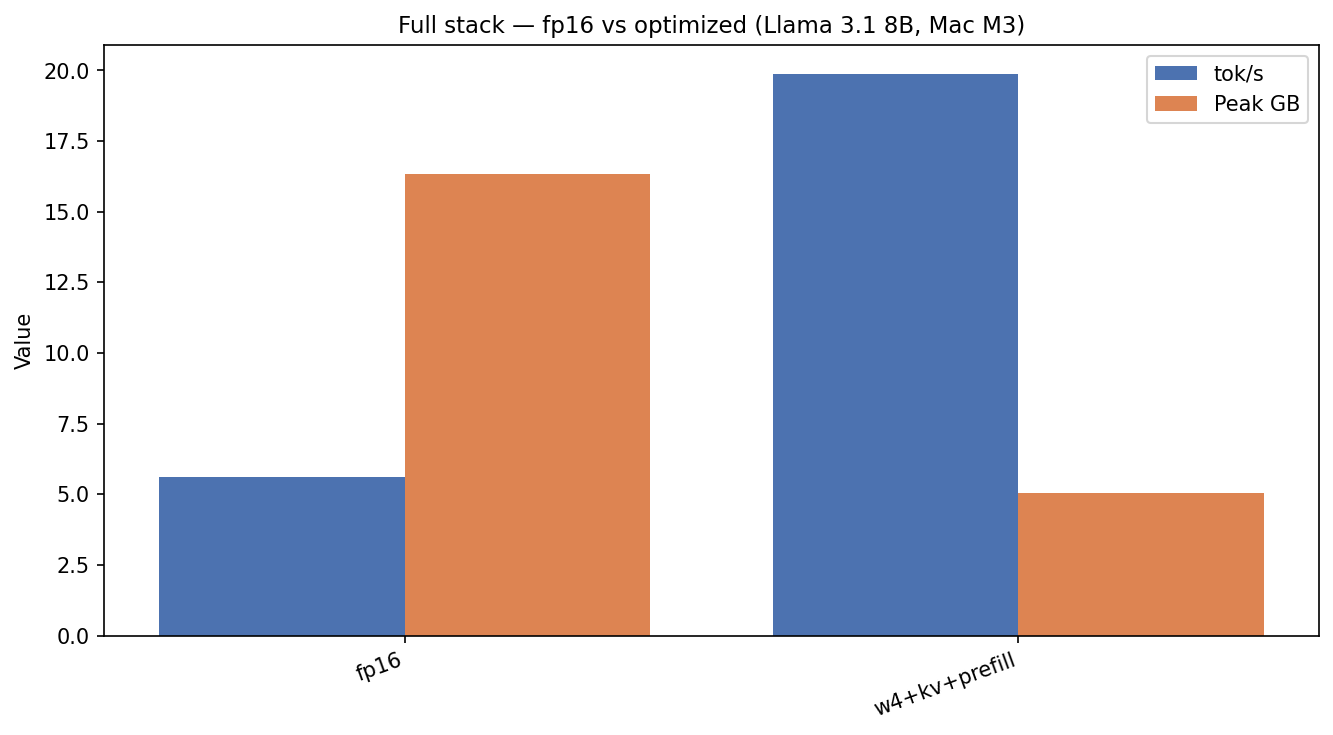
\includegraphics[width=0.98\linewidth]{figures/full_stack_llama.png}
  \caption{Mac M3, Llama~3.1~8B: FP16 versus the stacked 4-bit + KV + prefill recipe. Memory falls to \(\approx 31\%\) of baseline; decode rises \(\approx 3.55\times\)---enough that the machine remains a daily-use computer.}
  \label{fig:fullstack}
\end{figure}

\section{Open problems}
\label{sec:open}

\paragraph{Quality under compression on real tasks.}
Systems papers still under-report tool use, coding, and long-context reasoning at 4- and 2-bit. A cheap eval suite that travels with every GGUF/MLX quant would change local practice more than another 5\% kernel win.

\paragraph{Contended unified memory as a first-class model.}
Roofline assumes a GPU with private HBM. Unified DRAM, OS interference, and background apps make \(B_{\mathrm{mem}}\) a random variable. We need protocols that treat the laptop as a busy device, not an idle accelerator---including tests with a browser and IDE open.

\paragraph{When speculation fails.}
Acceptance \(\alpha\) is a property of the draft--target pair, temperature, and domain. Adaptive \(k\), draft routing, and ``disable speculation when \(\alpha\) drops'' should be default runtime features, especially when RAM is barely enough for two models.

\paragraph{Prefill as a product SLO.}
Industry dashboards over-index on decode tokens/s. RAG and agents die on TTFT. Chunked prefill, prefix caches, retrieve-less application design, and MInference-style sparse prefill need the same status as weight bits.

\paragraph{Cross-runtime equivalence.}
``4-bit'' in MLX, GPTQ, AWQ, and GGUF Q4\_K\_M are not the same random variable. A quant-tier ontology with shared perplexity probes would make runtime bake-offs honest.

\paragraph{Energy, thermals, and carbon of \emph{local} tokens.}
Tokens/s on a MacBook is eventually a skin-temperature problem; on a phone it is a battery problem~\citep{luccioni2024power}. Joules per token belong in local inference reports. Local serving also shifts carbon from datacenter to wall wart~\citep{patterson2021carbon}; that accounting is almost absent.

\paragraph{Phones, NPUs, and Windows ARM.}
Our measurements are Apple Silicon laptops. ExecuTorch / Hexagon / Neural Engine paths, thermal throttling, and 6--12\,GB phone budgets are the next empirical slice. Vendor on-device models~\citep{gunter2024apple} are closed enough that independent stacking studies are hard.

\paragraph{Heterogeneous local clusters.}
A household Mac mini plus a phone plus a spare PC is not DistServe, but disaggregated prefill/decode ideas~\citep{patel2024splitwise} might still apply. Almost no open harness studies that topology.

\section{Conclusion}
\label{sec:conclusion}

LLM inference optimization is not one trick, and it is not only a datacenter sport. On everyday devices it is a packing problem (does the model fit \emph{beside the operating system}?), a bandwidth problem (how many bytes per token?), a prefill problem (how long is the prompt you stuffed?), and only then a sequential-decode problem (can we verify several tokens at once?). The techniques in this survey attack those bottlenecks independently and can be stacked. The selling point is practical: a 24\,GB laptop can run a 7--9B assistant as a daily driver if you take 4-bit weights as default, insure KV for long \(T\), treat TTFT as the UX metric that RAG actually hits, and treat speculative decoding as a conditional bonus. The same catalog, read from the other end, is vLLM-style paging and disaggregated serving. We hope the related-work map, the equations, and the measurements make it obvious which end to open---and that ``it runs on my machine'' starts meaning the machine the reader already uses all day.


\begin{ack}
Benchmark numbers were collected with an open MLX harness on Apple Silicon. We thank the authors of the cited systems and the mlx-community and GGUF contributors who make comparable checkpoints public. Update this acknowledgment with funding and hardware donors before arXiv v1 if applicable.
\end{ack}

\bibliographystyle{plainnat}
\bibliography{references}

\newpage
\appendix
\section{Catalog checklist}
\label{app:catalog}

Table~\ref{tab:checklist} lists techniques covered in the body. Status tags refer to the companion Apple Silicon harness: \emph{measured} means a sweep exists; \emph{systems} means the method is standard in datacenter or local engines; \emph{architecture} means it is baked into the checkpoint; \emph{reference} means surveyed from the literature.

\begin{table*}[t]
  \centering
  \small
  \caption{Technique checklist (survey coverage).}
  \label{tab:checklist}
  \begin{tabular}{@{}llc@{}}
    \toprule
    Technique & Section & Typical status \\
    \midrule
    FP16 / BF16 baseline & \ref{sec:weights} & measured \\
    INT8 / 4-bit / 2-bit, GPTQ, AWQ, SmoothQuant & \ref{sec:weights} & measured / systems \\
    OmniQuant, QuaRot, SpinQuant, QuIP\#, AQLM, SpQR & \ref{sec:weights} & systems \\
    Activation quantization, QServe W4A8KV4 & \ref{sec:weights} & systems \\
    Pruning, distillation & \ref{sec:weights} & reference \\
    KV cache quantization, KIVI, KVQuant & \ref{sec:kv} & measured / systems \\
    GQA / MQA & \ref{sec:kv} & architecture \\
    PagedAttention & \ref{sec:kv}, \ref{sec:serving} & systems \\
    Prefix / prompt KV cache & \ref{sec:kv} & measured \\
    H2O, StreamingLLM, SnapKV, Quest, DuoAttention & \ref{sec:kv} & systems \\
    FlashAttention / tiled attention & \ref{sec:prefill} & measured (proxy) \\
    Prefill chunking, MInference & \ref{sec:prefill} & measured / systems \\
    Sparse attention, RoPE, YaRN, Mamba & \ref{sec:prefill} & architecture \\
    Speculative decoding, Medusa, EAGLE, SpecInfer & \ref{sec:decode} & measured / systems \\
    CUDA graphs / Metal capture, Deja Vu & \ref{sec:decode} & systems \\
    Continuous / static batching, Sarathi, DistServe, Splitwise & \ref{sec:serving} & systems \\
    Tensor / pipeline / expert parallel, EdgeMoE & \ref{sec:parallel} & systems \\
    Model-size ladder, Phi/TinyLlama/OpenELM/MobileLLM, MoE & \ref{sec:arch} & measured / reference \\
    LoRA / QLoRA / multi-LoRA & \ref{sec:lora} & systems \\
    Graph compile, offload, mmap, FlexGen, LLM-in-a-flash & \ref{sec:runtime} & systems \\
    MLX, llama.cpp, MLC, ExecuTorch, Ollama, PowerInfer & \ref{sec:runtime} & measured / systems \\
    RAG sizing, constrained decoding, early exit, tools & \ref{sec:app} & reference \\
    \bottomrule
  \end{tabular}
\end{table*}

\section{Reproducing the empirical slice}
\label{app:repro}

On Apple Silicon, with Python 3.10+ and Hugging Face access:
\begin{verbatim}
git clone <repo> LLM-Inference && cd LLM-Inference
./scripts/setup_env.sh && source .venv/bin/activate
./scripts/hf_login.sh
./scripts/run_article.sh 1 "Mac M3"   # weight quantization
./scripts/run_article.sh 5 "Mac M3"   # full stack
./scripts/run_article.sh 6 "Mac M3"   # speculative decoding
./scripts/run_article.sh 7 "Mac M3"   # context / RAG / prefix cache
\end{verbatim}
Each run writes schema-versioned JSON (median TTFT, tokens/s, peak GB). Tables in Section~\ref{sec:empirical} are medians from that schema. Large-model rows require a 64\,GB+ machine and \texttt{--include-large}.

\section{arXiv and NeurIPS usage notes}
\label{app:arxiv}

This source uses the official NeurIPS 2025 style with the \texttt{preprint} option. Authors are visible and the NeurIPS checklist is omitted. A broad on-device survey is a natural \textbf{arXiv} paper (\texttt{cs.LG}, cross-list \texttt{cs.CL}, \texttt{cs.DC}). NeurIPS main track is a poor fit unless the empirical protocol is framed as Datasets \& Benchmarks and cut to the page limit. A workshop on efficient or on-device ML is the more realistic conference path.


\end{document}
